\documentclass[14pt]{extbook}
\usepackage{multicol, enumerate, enumitem, hyperref, color, soul, setspace, parskip, fancyhdr} %General Packages
\usepackage{amssymb, amsthm, amsmath, bbm, latexsym, units, mathtools} %Math Packages
\everymath{\displaystyle} %All math in Display Style
% Packages with additional options
\usepackage[headsep=0.5cm,headheight=12pt, left=1 in,right= 1 in,top= 1 in,bottom= 1 in]{geometry}
\usepackage[usenames,dvipsnames]{xcolor}
\usepackage{dashrule}  % Package to use the command below to create lines between items
\newcommand{\litem}[1]{\item#1\hspace*{-1cm}\rule{\textwidth}{0.4pt}}
\pagestyle{fancy}
\lhead{Makeup Progress Quiz 3}
\chead{}
\rhead{Version A}
\lfoot{4315-3397}
\cfoot{}
\rfoot{Fall 2020}
\begin{document}

\begin{enumerate}
\litem{
Find the equation of the line described below. Write the linear equation as $ y=mx+b $ and choose the intervals that contain $m$ and $b$.\[ \text{Perpendicular to } 4 x + 3 y = 6 \text{ and passing through the point } (10, -8). \]\begin{enumerate}[label=\Alph*.]
\item \( m \in [0.97, 2.36] \hspace*{3mm} b \in [-16.5, -14.5] \)
\item \( m \in [0.07, 0.87] \hspace*{3mm} b \in [-16.5, -14.5] \)
\item \( m \in [0.07, 0.87] \hspace*{3mm} b \in [12.5, 17.5] \)
\item \( m \in [0.07, 0.87] \hspace*{3mm} b \in [-20, -17] \)
\item \( m \in [-1.41, -0.68] \hspace*{3mm} b \in [-4.5, 0.5] \)

\end{enumerate} }
\litem{
Solve the equation below. Then, choose the interval that contains the solution.\[ -13(-19x + 4) = -15(-12x -14) \]\begin{enumerate}[label=\Alph*.]
\item \( x \in [2.8, 5.9] \)
\item \( x \in [2.1, 2.6] \)
\item \( x \in [-3.4, -2.1] \)
\item \( x \in [-0.8, 0.8] \)
\item \( \text{There are no real solutions.} \)

\end{enumerate} }
\litem{
Solve the equation below. Then, choose the interval that contains the solution.\[ -10(8x -11) = -14(15x -16) \]\begin{enumerate}[label=\Alph*.]
\item \( x \in [1.11, 1.46] \)
\item \( x \in [0.75, 1.12] \)
\item \( x \in [1.95, 3.03] \)
\item \( x \in [-2.86, -2.24] \)
\item \( \text{There are no real solutions.} \)

\end{enumerate} }
\litem{
Solve the linear equation below. Then, choose the interval that contains the solution.\[ \frac{-7x -5}{4} - \frac{-6x -9}{8} = \frac{-9x -6}{5} \]\begin{enumerate}[label=\Alph*.]
\item \( x \in [-1.83, -0.52] \)
\item \( x \in [-13.5, -11.91] \)
\item \( x \in [1.38, 2.31] \)
\item \( x \in [-0.48, 0.72] \)
\item \( \text{There are no real solutions.} \)

\end{enumerate} }
\litem{
First, find the equation of the line containing the two points below. Then, write the equation as $ y=mx+b $ and choose the intervals that contain $m$ and $b$.\[ (-2, -10) \text{ and } (-3, 4) \]\begin{enumerate}[label=\Alph*.]
\item \( m \in [-14, -11] \hspace*{3mm} b \in [-40, -32] \)
\item \( m \in [-14, -11] \hspace*{3mm} b \in [34, 40] \)
\item \( m \in [-14, -11] \hspace*{3mm} b \in [-8, -3] \)
\item \( m \in [14, 16] \hspace*{3mm} b \in [39, 48] \)
\item \( m \in [-14, -11] \hspace*{3mm} b \in [3, 12] \)

\end{enumerate} }
\litem{
Write the equation of the line in the graph below in Standard form $Ax+By=C$. Then, choose the intervals that contain $A, B, \text{ and } C$.
\begin{center}
    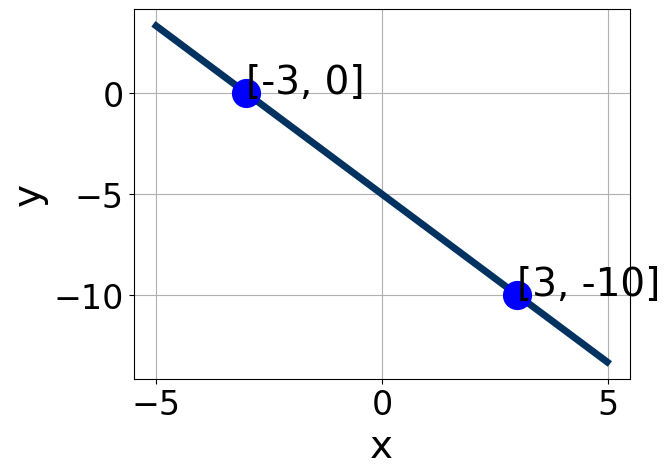
\includegraphics[width=0.5\textwidth]{../Figures/linearGraphToStandardCopyA.png}
\end{center}
\begin{enumerate}[label=\Alph*.]
\item \( A \in [3, 6], \hspace{3mm} B \in [2.04, 4], \text{ and } \hspace{3mm} C \in [-19, -12] \)
\item \( A \in [-5, 0], \hspace{3mm} B \in [-3.53, -2.92], \text{ and } \hspace{3mm} C \in [8, 18] \)
\item \( A \in [3, 6], \hspace{3mm} B \in [-3.53, -2.92], \text{ and } \hspace{3mm} C \in [8, 18] \)
\item \( A \in [0.67, 3.67], \hspace{3mm} B \in [-1.47, 0.35], \text{ and } \hspace{3mm} C \in [4, 11] \)
\item \( A \in [0.67, 3.67], \hspace{3mm} B \in [0.37, 1.26], \text{ and } \hspace{3mm} C \in [-5, -3] \)

\end{enumerate} }
\litem{
Write the equation of the line in the graph below in Standard form $Ax+By=C$. Then, choose the intervals that contain $A, B, \text{ and } C$.
\begin{center}
    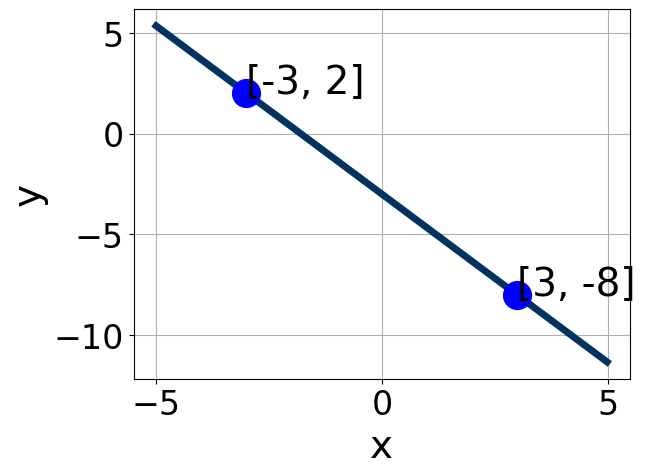
\includegraphics[width=0.5\textwidth]{../Figures/linearGraphToStandardA.png}
\end{center}
\begin{enumerate}[label=\Alph*.]
\item \( A \in [-6.5, -3.5], \hspace{3mm} B \in [-4.44, -2.94], \text{ and } \hspace{3mm} C \in [8, 16] \)
\item \( A \in [-2.2, 3.6], \hspace{3mm} B \in [-1.79, -0.02], \text{ and } \hspace{3mm} C \in [0, 4] \)
\item \( A \in [-2.2, 3.6], \hspace{3mm} B \in [-0.43, 1.96], \text{ and } \hspace{3mm} C \in [-6, -2] \)
\item \( A \in [2.6, 6.8], \hspace{3mm} B \in [-4.44, -2.94], \text{ and } \hspace{3mm} C \in [8, 16] \)
\item \( A \in [2.6, 6.8], \hspace{3mm} B \in [2.62, 4.5], \text{ and } \hspace{3mm} C \in [-12, -8] \)

\end{enumerate} }
\litem{
First, find the equation of the line containing the two points below. Then, write the equation as $ y=mx+b $ and choose the intervals that contain $m$ and $b$.\[ (9, -6) \text{ and } (-11, -5) \]\begin{enumerate}[label=\Alph*.]
\item \( m \in [-0.06, -0.05] \hspace*{3mm} b \in [5.15, 5.76] \)
\item \( m \in [-0.06, -0.05] \hspace*{3mm} b \in [-15.53, -14.69] \)
\item \( m \in [-0.06, -0.05] \hspace*{3mm} b \in [-5.63, -5.32] \)
\item \( m \in [-0.04, 0.14] \hspace*{3mm} b \in [-4.92, -4.38] \)
\item \( m \in [-0.06, -0.05] \hspace*{3mm} b \in [5.91, 6.37] \)

\end{enumerate} }
\litem{
Find the equation of the line described below. Write the linear equation as $ y=mx+b $ and choose the intervals that contain $m$ and $b$.\[ \text{Parallel to } 8 x + 5 y = 12 \text{ and passing through the point } (-5, 2). \]\begin{enumerate}[label=\Alph*.]
\item \( m \in [-2.52, -1.58] \hspace*{3mm} b \in [4.6, 6.4] \)
\item \( m \in [0.6, 2.35] \hspace*{3mm} b \in [9, 10.2] \)
\item \( m \in [-2.52, -1.58] \hspace*{3mm} b \in [6.4, 8] \)
\item \( m \in [-2.52, -1.58] \hspace*{3mm} b \in [-6.1, -3.3] \)
\item \( m \in [-0.84, 0.09] \hspace*{3mm} b \in [-6.1, -3.3] \)

\end{enumerate} }
\litem{
Solve the linear equation below. Then, choose the interval that contains the solution.\[ \frac{9x + 8}{4} - \frac{4x + 3}{3} = \frac{9x -5}{5} \]\begin{enumerate}[label=\Alph*.]
\item \( x \in [-0.6, 1.3] \)
\item \( x \in [11, 11.4] \)
\item \( x \in [1.3, 2.9] \)
\item \( x \in [3.8, 5.8] \)
\item \( \text{There are no real solutions.} \)

\end{enumerate} }
\end{enumerate}

\end{document}